% =====================================================================
%  en-nlp.tex  --  48 x 36 in landscape academic poster
%  Bounded Calibration under Fuzzy Evidence
%  ACL / EMNLP / NAACL style.  XeLaTeX.
% =====================================================================
\documentclass[10pt]{article}

\usepackage{fontspec}
\setmainfont{Helvetica Neue}[
  BoldFont={Helvetica Neue Bold},
  ItalicFont={Helvetica Neue Italic},
  BoldItalicFont={Helvetica Neue Bold Italic}]
\setmonofont{Menlo}[Scale=0.90]
\usepackage{unicode-math}
\setmathfont{STIX Two Math}

\usepackage{geometry}
\geometry{paperwidth=1219.2mm,paperheight=914.4mm,margin=0mm}
\geometry{left=60pt,right=60pt,top=338pt,bottom=60pt,noheadfoot}

\usepackage[table]{xcolor}
\usepackage{amsmath}
\usepackage{array}
\usepackage{booktabs}
\usepackage{tabularx}
\usepackage{tikz}
\usetikzlibrary{calc,positioning,arrows.meta,shapes.misc,fit,backgrounds}
\usepackage{tcolorbox}
\tcbuselibrary{skins,breakable}
\usepackage{enumitem}
\usepackage{qrcode}

% ---------------------------------------------------------------- palette
\definecolor{navy}{HTML}{0B1F33}
\definecolor{teal}{HTML}{0E7C86}
\definecolor{coral}{HTML}{D95D39}
\definecolor{ssered}{HTML}{A6192E}
\definecolor{lgray}{HTML}{F3F5F7}
\definecolor{mgray}{HTML}{D5DCE3}
\definecolor{slate}{HTML}{44566B}
\definecolor{muted}{HTML}{6A7887}
\definecolor{tealL}{HTML}{E8F2F3}
\definecolor{coralL}{HTML}{FBEDE7}
\definecolor{titleaccent}{HTML}{7FC6CE}

% ---------------------------------------------------------------- fonts
\newcommand{\fsBody}{\fontsize{22.5}{27}\selectfont}
\newcommand{\fsSmall}{\fontsize{19}{23.5}\selectfont}
\newcommand{\fsFine}{\fontsize{17}{21}\selectfont}
\newcommand{\fsTiny}{\fontsize{15}{18.5}\selectfont}
\newcommand{\trk}[1]{{\addfontfeatures{LetterSpace=13}\MakeUppercase{#1}}}
\newcommand{\trks}[1]{{\addfontfeatures{LetterSpace=9}\MakeUppercase{#1}}}

\newcommand{\chip}[2]{{\setlength{\fboxsep}{3.5pt}%
  \raisebox{0.12em}{\colorbox{#2}{\color{white}\fontsize{12.5}{12.5}\selectfont\bfseries\trk{#1}}}}}

% ---------------------------------------------------------------- lengths
\newlength{\gut}\setlength{\gut}{16mm}
\newlength{\colw}\setlength{\colw}{\dimexpr(\textwidth-3\gut)/4\relax}

% ---------------------------------------------------------------- headings
\newcommand{\sechead}[3]{%  #1 number, #2 title, #3 tagline
  \par\addvspace{6pt}%
  \noindent{\setlength{\fboxsep}{0pt}%
    \colorbox{seccolor}{%
      \begin{minipage}{\linewidth}%
        \vspace{8.5pt}\hspace*{14pt}%
        {\parfillskip=14pt\relax
        {\color{white}\fontsize{28}{31}\selectfont\bfseries
          {\color{white!55!seccolor}\trk{#1}}\hspace{10pt}\trk{#2}}%
        \hfill{\color{white!72!seccolor}\fontsize{16}{18}\selectfont\itshape #3}\par}%
        \vspace{8.5pt}%
      \end{minipage}}}%
  \par\addvspace{9pt}%
}

\newcommand{\subhead}[1]{%
  \par\addvspace{11pt}\noindent
  {\color{navy}\fontsize{21}{24}\selectfont\bfseries\trks{#1}}%
  \par\nobreak\vspace{2.5pt}%
  {\color{mgray}\hrule height 1pt}%
  \par\addvspace{8pt}%
}

% ---------------------------------------------------------------- equation panel
\newtcolorbox{eqbox}[1][]{enhanced, colback=lgray, colframe=lgray, boxrule=0pt,
  arc=2pt, sharp corners=south, left=9pt, right=9pt, top=5pt, bottom=5pt,
  before skip=7pt, after skip=7pt, fontupper=\fontsize{21.5}{26}\selectfont, #1}

\newcommand{\eqtag}[1]{{\color{muted}\fontsize{15.5}{15.5}\selectfont(#1)}}

% ---------------------------------------------------------------- lists
\setlist[itemize]{label={\raisebox{0.28em}{\color{teal}\rule{7pt}{7pt}}},
  leftmargin=20pt, labelsep=9pt, topsep=3pt, itemsep=3.5pt, parsep=0pt, partopsep=0pt}
\setlist[enumerate]{leftmargin=26pt, labelsep=8pt, topsep=3pt, itemsep=4pt, parsep=0pt}

% ---------------------------------------------------------------- tikz styles
\tikzset{
  arrow/.style={-{Stealth[length=9pt,width=7pt]}, line width=2.2pt, draw=slate},
  thinarrow/.style={-{Stealth[length=7pt,width=5.5pt]}, line width=1.4pt, draw=slate},
  panel/.style={rounded corners=4pt, line width=1pt},
}

\setlength{\parindent}{0pt}
\setlength{\parskip}{5pt plus 1pt}
\AtBeginDocument{%
  \setlength{\abovedisplayskip}{3pt}\setlength{\belowdisplayskip}{3pt}%
  \setlength{\abovedisplayshortskip}{2pt}\setlength{\belowdisplayshortskip}{2pt}%
  \raggedright\emergencystretch=2em\hyphenpenalty=400}

\begin{document}
\pagestyle{empty}

% =====================================================================
%  HEADER (full bleed, 110 mm = 312 pt)
% =====================================================================
\begin{tikzpicture}[remember picture, overlay, x=1pt, y=1pt]
  \coordinate (NW) at (current page.north west);
  \fill[navy] (NW) rectangle ++(\paperwidth,-312pt);
  \fill[ssered] ($(NW)+(0,-308pt)$) rectangle ++(\paperwidth,-4pt);

  \node[anchor=base west, inner sep=0pt, text=titleaccent,
        font=\fontsize{17}{17}\selectfont\addfontfeatures{LetterSpace=22}]
    at ($(NW)+(60pt,-50pt)$) {MULTI-AGENT SYSTEMS \ \ $\cdot$ \ \ EQUITY VALUATION \ \ $\cdot$ \ \ NLP FOR FINANCE};

  \node[anchor=base west, inner sep=0pt, text=white,
        font=\fontsize{83}{87}\selectfont\bfseries]
    at ($(NW)+(58pt,-126pt)$) {Bounded Calibration under Fuzzy Evidence:};
  \node[anchor=base west, inner sep=0pt, text=titleaccent,
        font=\fontsize{83}{87}\selectfont\bfseries]
    at ($(NW)+(58pt,-212pt)$) {Hierarchical MoE and Multi-Agent Review for Valuation};

  \node[anchor=base west, inner sep=0pt, text=white,
        font=\fontsize{29}{29}\selectfont\bfseries]
    at ($(NW)+(60pt,-264pt)$) {Yingzhou Chen\textsuperscript{\dag}, Boyi Song\textsuperscript{\dag,*}, Shenyi Sun\textsuperscript{\dag}};
  \node[anchor=base west, inner sep=0pt, text=white!82,
        font=\fontsize{19}{19}\selectfont]
    at ($(NW)+(60pt,-296pt)$) {China Securities Index Co., Ltd.\ (CSI), Shanghai, China \quad\textperiodcentered\quad
    \textsuperscript{\dag}\,Equal contribution \quad\textperiodcentered\quad
    \textsuperscript{*}\,Corresponding: Boyi Song, bysong@sse.com.cn};

  \node[anchor=north west, inner sep=0pt, text=white!70, align=left,
        font=\fontsize{21}{26.5}\selectfont\itshape, text width=900pt]
    at ($(NW)+(2260pt,-140pt)$)
    {Enterprise valuation is a conditional nonlinear mapping under fuzzy evidence. Multi-agent review is not an oracle but a bounded, auditable parameter updater, moving the system from human-set parameters to agent-proposed, system-learned calibration.};
  \node[anchor=north west, inner sep=0pt, text=titleaccent,
        font=\fontsize{12}{12.5}\selectfont\addfontfeatures{LetterSpace=16}]
    at ($(NW)+(2274pt,-116pt)$) {THESIS};
  % ---- QR block (right)
  \fill[white, rounded corners=3pt] ($(NW)+(3248pt,-20pt)$) rectangle ($(NW)+(3404pt,-176pt)$);
  \node[anchor=north east, inner sep=0pt] (qr) at ($(NW)+(\paperwidth-64pt,-32pt)$)
    {\qrcode[height=132pt]{https://github.com/Boyee2022/ipo-valuation-index}};
  \node[anchor=north east, inner sep=0pt, text=teal!55!white,
        font=\fontsize{13.5}{14}\selectfont\addfontfeatures{LetterSpace=14}]
    at ($(NW)+(\paperwidth-62pt,-190pt)$) {CODE \ \& \ ARTIFACTS};
  \node[anchor=north east, inner sep=0pt, text=white!80, align=right,
        font=\fontsize{14}{16.5}\selectfont]
    at ($(NW)+(\paperwidth-62pt,-210pt)$) {github.com/Boyee2022/\\ipo-valuation-index};

\end{tikzpicture}

% =====================================================================
%  HERO  --  Figure 1, full-width pipeline
% =====================================================================
\noindent\begin{tikzpicture}[x=1pt, y=-1pt, baseline=(current bounding box.north)]
  \fill[lgray, rounded corners=6pt] (0,0) rectangle (3334,262);

  \node[anchor=north west, inner sep=0pt, text=muted,
        font=\fontsize{14}{15}\selectfont\addfontfeatures{LetterSpace=13}]
    at (24,16) {FIGURE 1 \ \ $\cdot$ \ \ END-TO-END PIPELINE: FROM CONSTITUENTS TO AN AUDITABLE VALUATION-LEVEL SERIES};

  % --- card macro: name, x, fill, draw, text block
  \newcommand{\stagecard}[5]{%
    \node[panel, fill=#3, draw=#4, minimum width=505pt, minimum height=146pt,
          inner sep=0pt, anchor=north west] (#1) at (#2,42) {};%
    \node[anchor=north west, inner sep=0pt, text width=471pt, align=left]
      at ($(#1.north west)+(17pt,-13pt)$) {#5};%
  }

  \stagecard{b0}{14}{white}{mgray}{%
    {\color{muted}\fontsize{13}{14}\selectfont\addfontfeatures{LetterSpace=15}01}\\[7pt]
    {\color{navy}\fontsize{26}{29}\selectfont\bfseries INDEX INPUT}\\[9pt]
    {\color{slate}\fontsize{19}{23}\selectfont 5 CSI indices, 2,201 SSE Composite constituents; public disclosures, comparables, quotes and news.}}

  \stagecard{b1}{577}{tealL}{teal!55}{%
    {\color{teal}\fontsize{13}{14}\selectfont\addfontfeatures{LetterSpace=15}02}\\[7pt]
    {\color{navy}\fontsize{26}{29}\selectfont\bfseries EVIDENCE PACK}\\[9pt]
    {\color{slate}\fontsize{19}{23}\selectfont Four-level resolution ladder, Layer-0 gate, six-stage lifecycle; skipped stocks leave the index.}}

  \stagecard{b2}{1140}{navy}{navy}{%
    {\color{titleaccent}\fontsize{13}{14}\selectfont\addfontfeatures{LetterSpace=15}03}\\[7pt]
    {\color{white}\fontsize{26}{29}\selectfont\bfseries VALUATION ENGINE}\\[9pt]
    {\color{white!82}\fontsize{19}{23}\selectfont Seven methods gated by lifecycle and availability; per-stock value, interval and confidence.}}

  \stagecard{b3}{1703}{coralL}{coral!60}{%
    {\color{coral}\fontsize{13}{14}\selectfont\addfontfeatures{LetterSpace=15}04}\\[7pt]
    {\color{navy}\fontsize{26}{29}\selectfont\bfseries BOUNDED REVIEW}\\[9pt]
    {\color{slate}\fontsize{19}{23}\selectfont 3 experts $\rightarrow$ evidence gates $\rightarrow$ chief $\rightarrow$ accept / clamp / reject. Deltas only, never a price.}}

  \stagecard{b4}{2266}{tealL}{teal!55}{%
    {\color{teal}\fontsize{13}{14}\selectfont\addfontfeatures{LetterSpace=15}05}\\[7pt]
    {\color{navy}\fontsize{26}{29}\selectfont\bfseries COMPOSITION}\\[9pt]
    {\color{slate}\fontsize{19}{23}\selectfont Level $=P^{\mathrm{idx}}\times$ index-weighted mean of $V_i/P_i$; three scenario levels, scale-consistent by construction.}}

  \stagecard{b5}{2829}{white}{mgray}{%
    {\color{muted}\fontsize{13}{14}\selectfont\addfontfeatures{LetterSpace=15}06}\\[7pt]
    {\color{navy}\fontsize{26}{29}\selectfont\bfseries REPORT + AUDIT}\\[9pt]
    {\color{slate}\fontsize{19}{23}\selectfont 11-section report, 8 machine checks, per-stock \texttt{shadow.json}, batch snapshot, rollback log.}}

  \node[panel, draw=coral, line width=3pt, minimum width=505pt, minimum height=146pt,
        inner sep=0pt, anchor=north west] at (1703,42) {};

  \foreach \i in {0,1,2,3,4}{%
    \pgfmathtruncatemacro{\j}{\i+1}%
    \draw[arrow] (b\i.east) -- (b\j.west);
  }

  \draw[-{Bar[width=13pt]}, dashed, line width=2pt, draw=coral]
    (b5.south) -- (3091.5,216) -- (1392.5,216) -- (b2.south);
  \node[anchor=north, text=coral, font=\fontsize{17}{17}\selectfont]
    at (2241,222) {$e_i=V_i/P_i-1$ \ \ diagnostic only \ \ $\cdot$ \ \ never back-propagated, never a label};
\end{tikzpicture}


% ---- column bodies (also measured below) ----
\newcommand{\colA}{%


% ---------------------------------------------------------------- COL 1
{\colorlet{seccolor}{teal}%
\sechead{01}{Motivation}{why synthesize an index from valuations}}

Every index level is a weighted sum of prices. This system replaces the price input with a per-constituent valuation, so the aggregate expresses what companies are worth relative to fundamentals rather than what they trade at.

\subhead{What the construction must deliver}
\begin{itemize}
\item A per-stock value with an interpretable interval, not a point forecast.
\item A scale-consistent rule: if every stock is valued at $k\times$ its price, the level must scale by $k$.
\item Parameter changes that are reviewable, bounded and reversible.
\end{itemize}

\subhead{Three fuzziness}
\begin{tcolorbox}[enhanced, frame hidden, colback=white, boxrule=0pt,
  borderline west={4.5pt}{0pt}{teal}, left=16pt, right=10pt, top=6pt, bottom=6pt,
  before skip=5pt, after skip=2pt, fontupper=\fontsize{19}{23}\selectfont]
{\color{teal}\fontsize{14.5}{15}\selectfont\bfseries\trk{Input}}\\[2pt]
Mixed reporting definitions, missing comparables, new listings and ST names, non-point-in-time snapshots. \emph{Handling:} four-level ladder (statement $\rightarrow$ collection $\rightarrow$ query $\rightarrow$ default); missing inputs are skipped or lose confidence.
\end{tcolorbox}
\begin{tcolorbox}[enhanced, frame hidden, colback=white, boxrule=0pt,
  borderline west={4.5pt}{0pt}{teal}, left=16pt, right=10pt, top=6pt, bottom=6pt,
  before skip=2pt, after skip=2pt, fontupper=\fontsize{19}{23}\selectfont]
{\color{teal}\fontsize{14.5}{15}\selectfont\bfseries\trk{Model}}\\[2pt]
DCF, comparables, sentiment, RIM, DDM, rNPV and SOTP have disjoint domains; the lifecycle label is itself error-prone. \emph{Handling:} Layer-0 admissibility gate, six lifecycle stages, method routing, renormalisation over what remains available.
\end{tcolorbox}
\begin{tcolorbox}[enhanced, frame hidden, colback=white, boxrule=0pt,
  borderline west={4.5pt}{0pt}{coral}, left=16pt, right=10pt, top=6pt, bottom=6pt,
  before skip=2pt, after skip=4pt, fontupper=\fontsize{19}{23}\selectfont]
{\color{coral}\fontsize{14.5}{15}\selectfont\bfseries\trk{Target}}\\[2pt]
No ground-truth value; price is not value; the index close is not the answer; accurate, stable, explainable and auditable conflict. \emph{Handling:} disagreement with price is diagnosed, never back-propagated.
\end{tcolorbox}

\begin{tcolorbox}[enhanced, frame hidden, colback=lgray, boxrule=0pt,
  borderline west={5pt}{0pt}{ssered}, left=14pt, right=11pt, top=7pt, bottom=7pt,
  before skip=6pt, after skip=2pt, fontupper=\fontsize{20}{24.5}\selectfont]
{\color{ssered}\fontsize{17}{19}\selectfont\bfseries\trks{No price labels.}}\ \ We do not minimise $\sum_i (V_i-P_i)^2$. The residual $e_i=V_i/P_i-1$ is reported and decomposed by industry, but it never becomes a supervision signal: fitting the close would learn noise, liquidity and sentiment into the value.
\end{tcolorbox}

\begin{tcolorbox}[enhanced, frame hidden, colback=navy, boxrule=0pt,
  borderline west={5pt}{0pt}{coral}, left=15pt, right=12pt, top=8pt, bottom=8pt,
  before skip=6pt, after skip=4pt, fontupper=\fontsize{20}{25}\selectfont]
{\color{titleaccent}\fontsize{14}{15}\selectfont\addfontfeatures{LetterSpace=14}RESEARCH QUESTION}\\[3pt]
{\color{white}How can an LLM reviewer improve a valuation engine's calibration when no label exists --- without letting the model price assets freely?}
\end{tcolorbox}

\subhead{Contributions}
\begin{itemize}[itemsep=4pt]
\item \textbf{Problem.} Valuation as a conditional nonlinear mapping under fuzzy evidence; calibration as constrained optimisation over a feasible parameter set, with no target label.
\item \textbf{Model.} A hierarchical mixture of experts over lifecycle $\times$ method, fuzzy $\alpha$-cut intervals, three pooling semantics, and a scale-consistent index composition rule.
\item \textbf{Protocol and evidence.} Expert review formalised as a bounded, auditable trust-region update; a shipped system (five indices, 2,201 constituents) and an evaluation protocol that needs no ground truth.
\end{itemize}

{\colorlet{seccolor}{navy}%
\sechead{02}{Method}{hierarchical MoE, fuzzy weights, composition}}

The engine, not the language model, produces value. Valuation methods are the experts; the lifecycle stage is the upper gate; the LLM may only edit parameters, and only inside bounds.

\begin{eqbox}
\begin{equation*}\tag*{\eqtag{1}}
F(x;\Theta)=\sum_{z\in Z}p(z\mid x)\sum_{m\in M}w_{m\mid z}(x)\,f_{m,z}(x;\theta_{m,z})
\end{equation*}
\end{eqbox}

\begin{eqbox}
\begin{equation*}\tag*{\eqtag{2}}
w_{m\mid z}(x)=\frac{a_m(x)\,\mu_{m,z}(x)\,e^{\gamma_m}}{\sum_{j\in M}a_j(x)\,\mu_{j,z}(x)\,e^{\gamma_j}}
\end{equation*}
\end{eqbox}

$a_m\in\{0,1\}$ is hard availability from data and the Layer-0 gate; $\mu_{m,z}\in[0,1]$ is soft applicability; $\gamma_m$ is a method prior. In the shipped engine $p(z\mid x)$ is a near one-hot route over six stages (structural evidence outranks the sign of earnings), $\gamma_m$ stands in for the fixed three-way weights, and $\mu$ remains rule-based. The gate is interpretable but subjective, and we report it as a design choice rather than a fitted quantity.

\subhead{Three pooling semantics}
\begin{itemize}[itemsep=3pt]
\item \textbf{Linear (shipped)} $\ \sum_m w_m v_m$. No disagreement penalty; a high multiple can dominate.
\item \textbf{Log} $\ \exp(\sum_m w_m\ln v_m)$. The AM--GM gap acts as a disagreement penalty; unstable near zero.
\item \textbf{Product of experts} $\ p(V\mid e)\propto\prod_m p_m(V\mid e)^{w_m}$. Precision-weighted, but needs calibrated likelihoods; correlated experts make it overconfident.
\end{itemize}
We treat the three as an ablation, not as a claim about which is best.

}
\newcommand{\colB}{%


% ---------------------------------------------------------------- COL 2
\subhead{Fuzzy weights and $\alpha$-cuts}

\chip{paper extension}{coral}\ \ Weights and method values are lifted to fuzzy numbers. The $\alpha$-cut is a fractional program, solved exactly for $M\le 4$ by enumerating weight-box vertices (or via a Charnes--Cooper transform); we report $[V]_{0.1},[V]_{0.5},[V]_{0.9}$ and defuzzify at the median.

\begin{eqbox}[fontupper=\fontsize{19.6}{24}\selectfont]
\begin{equation*}\tag*{\eqtag{3}}
[V]_\alpha=\left\{\frac{\sum_m w_m v_m}{\sum_m w_m}:\ w_m\in[w_m]_\alpha,\ v_m\in[v_m]_\alpha\right\},\qquad
\hat V=\tfrac12\left(V^-_{0.5}+V^+_{0.5}\right)
\end{equation*}
\end{eqbox}

Status: paper extension; the shipped system reports crisp weights with Monte-Carlo and scenario intervals.

\subhead{Index composition}

\begin{eqbox}
\begin{equation*}\tag*{\eqtag{4}}
V^{\mathrm{idx}}=P^{\mathrm{idx}}\cdot\frac{\sum_i w_i\left(V_i/P_i\right)}{\sum_i w_i},
\qquad
V^{\mathrm{pw}}=P^{\mathrm{idx}}\cdot\frac{\sum_i w_iV_i}{\sum_i w_iP_i}
\end{equation*}
\end{eqbox}

\chip{shipped}{teal}\ \ Scale consistency: if $V_i=kP_i$ for all $i$, then $V^{\mathrm{idx}}=kP^{\mathrm{idx}}$. Skipped stocks leave both numerator and denominator. Scenario levels apply the same weights to per-stock interval ends, so level and width are read together. The price-weighted variant $V^{\mathrm{pw}}$ is a control only: it over-weights high-priced stocks by construction.


% ---- Figure 2 : hierarchical gate
\vspace{2pt}
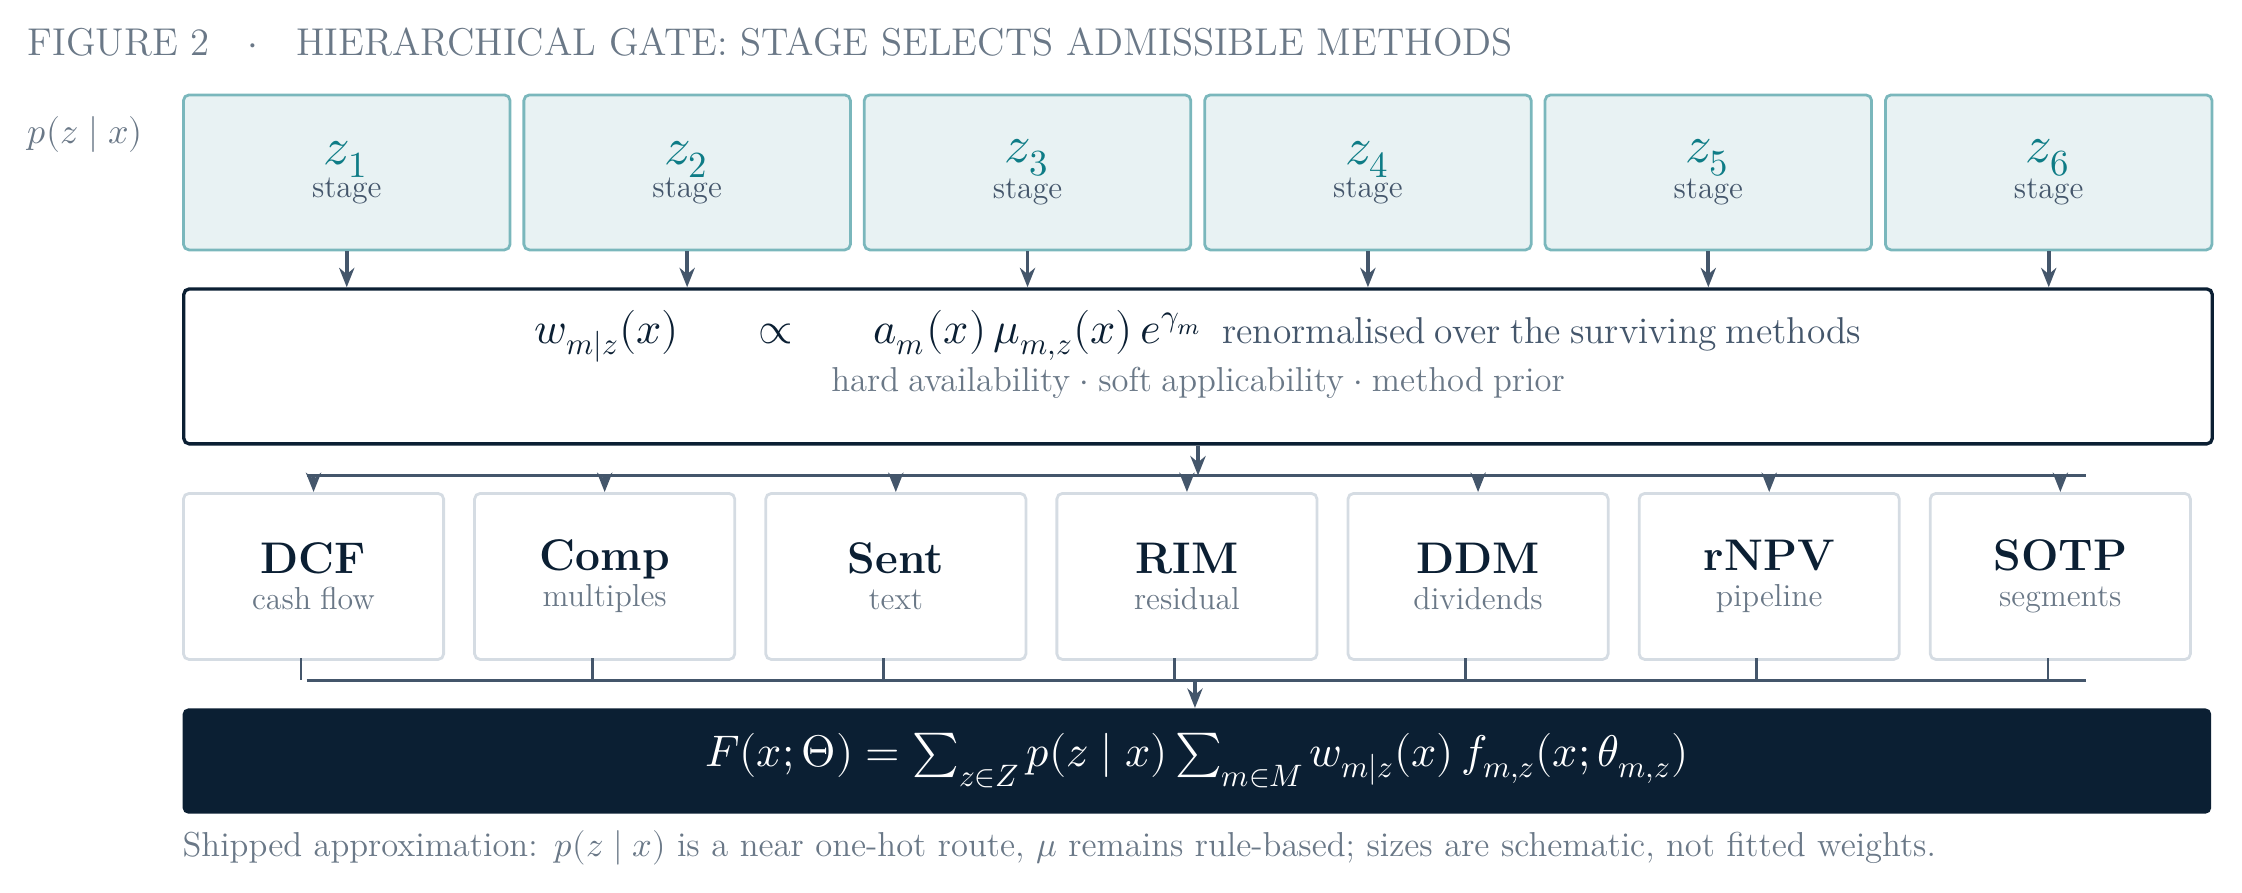
\begin{tikzpicture}[x=1pt, y=-1pt, baseline=(current bounding box.north)]
  \node[anchor=north west, inner sep=0pt, text=muted,
        font=\fontsize{14}{15}\selectfont\addfontfeatures{LetterSpace=12}]
    at (0,0) {FIGURE 2 \ \ $\cdot$ \ \ HIERARCHICAL GATE: STAGE SELECTS ADMISSIBLE METHODS};

  \node[anchor=north west, inner sep=0pt, text=muted, font=\fontsize{13}{15}\selectfont]
    at (0,32) {$p(z\mid x)$};

  \foreach \i in {0,...,5}{%
    \node[draw=teal!55, fill=tealL, rounded corners=2pt, line width=1pt,
          text width=108pt, inner sep=5pt, minimum height=56pt, anchor=north west, align=center]
      (z\i) at ({56+\i*123},24)
      {{\color{teal}\fontsize{19}{21}\selectfont\bfseries $z_{\the\numexpr\i+1}$}\\[0pt]
       {\color{slate}\fontsize{11.5}{13}\selectfont stage}};
    \draw[thinarrow] (z\i.south) -- (z\i.south |- {0,94});
  }

  \node[fill=white, draw=navy, line width=1.2pt, rounded corners=2pt, inner sep=0pt,
        minimum width=733pt, minimum height=56pt, anchor=north west, align=center]
    (gate) at (56,94) {};
  \node[anchor=north, inner sep=0pt, align=center, text width=700pt]
    at ($(gate.north)+(0,-8pt)$)
    {{\color{navy}\fontsize{16}{19}\selectfont $w_{m\mid z}(x)\propto a_m(x)\,\mu_{m,z}(x)\,e^{\gamma_m}$\ \ \color{slate}\fontsize{13.5}{16}\selectfont renormalised over the surviving methods}\\[1pt]
     {\color{muted}\fontsize{12.5}{15}\selectfont hard availability $\cdot$ soft applicability $\cdot$ method prior}};

  % bus to methods
  \draw[thinarrow] (gate.south) -- (gate.south |- {0,162});
  \draw[slate, line width=1.2pt] (101,162) -- (744,162);

  \foreach \i/\nm/\rl in {0/DCF/cash flow,1/Comp/multiples,2/Sent/text,3/RIM/residual,4/DDM/dividends,5/rNPV/pipeline,6/SOTP/segments}{%
    \node[draw=mgray, fill=white, rounded corners=2pt, line width=1pt,
          text width=86pt, inner sep=4pt, minimum height=60pt, anchor=north west, align=center]
      (m\i) at ({56+\i*105.2},168)
      {{\color{navy}\fontsize{16}{18}\selectfont\bfseries \nm}\\[1pt]
       {\color{muted}\fontsize{11.5}{13}\selectfont \rl}};
    \draw[thinarrow] (m\i.north |- {0,162}) -- (m\i.north);
  }

  % collector to output
  \draw[slate, line width=1.2pt] (101,236) -- (744,236);
  \foreach \i in {0,...,6}{%
    \draw[slate, line width=1pt] ({99+\i*105.2},228) -- ({99+\i*105.2},236);
  }
  \draw[thinarrow] (422,236) -- (422,246);

  \node[fill=navy, rounded corners=2pt, inner sep=0pt, minimum width=733pt, minimum height=38pt,
        anchor=north west, align=center] (out) at (56,246) {};
  \node[anchor=north, inner sep=0pt, text=white, font=\fontsize{16}{18}\selectfont]
    at ($(out.north)+(0,-9pt)$)
    {$F(x;\Theta)=\sum_{z\in Z}p(z\mid x)\sum_{m\in M}w_{m\mid z}(x)\,f_{m,z}(x;\theta_{m,z})$};

  \node[anchor=north west, inner sep=0pt, text=muted, font=\fontsize{12.5}{15}\selectfont, text width=725pt]
    at (56,290) {Shipped approximation: $p(z\mid x)$ is a near one-hot route, $\mu$ remains rule-based; sizes are schematic, not fitted weights.};
\end{tikzpicture}

% ---------------------------------------------------------------- section 3
{\colorlet{seccolor}{coral}%
\sechead{03}{Bounded Agent Review}{three experts, gates, rollback}}

The LLM never emits a price. Three specialists each see one evidence domain and may propose only their own parameters; a chief reviewer accepts, clamps or rejects. Experts never see the index level or a price target, so there is nothing to optimise toward.

% ---- Figure 3 : protocol
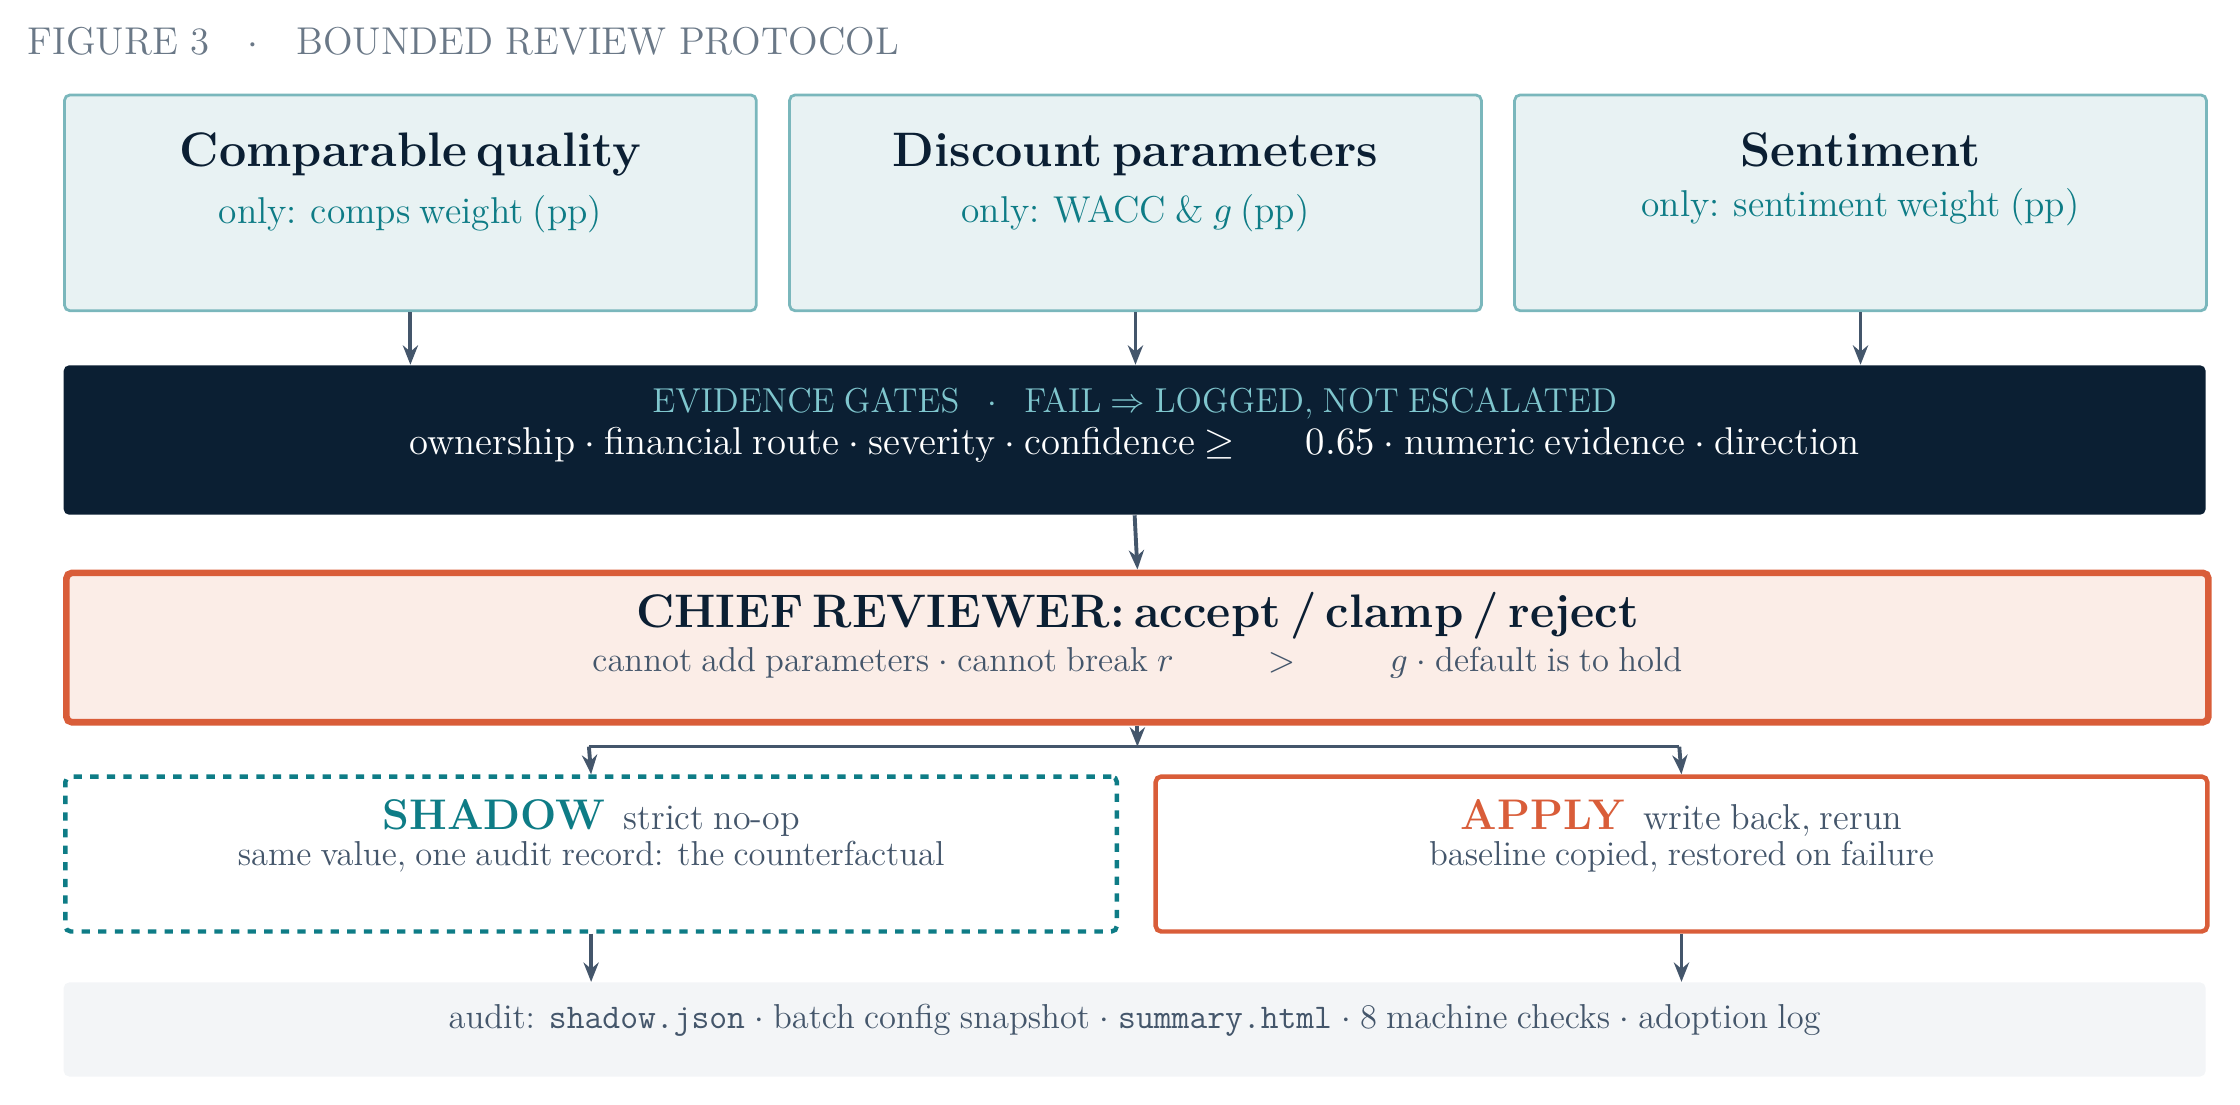
\begin{tikzpicture}[x=1pt, y=-1pt, baseline=(current bounding box.north)]
  \node[anchor=north west, inner sep=0pt, text=muted,
        font=\fontsize{14}{15}\selectfont\addfontfeatures{LetterSpace=12}]
    at (0,0) {FIGURE 3 \ \ $\cdot$ \ \ BOUNDED REVIEW PROTOCOL};

  \foreach \i/\nm/\prm in {0/Comparable quality/comps weight (pp),1/Discount parameters/WACC \& $g$ (pp),2/Sentiment/sentiment weight (pp)}{%
    \node[draw=teal!55, fill=tealL, rounded corners=2pt, line width=1pt, inner sep=0pt,
          minimum width=250pt, minimum height=78pt, anchor=north west, align=center]
      (e\i) at ({13+\i*262},24) {};
    \node[anchor=north, inner sep=0pt, text width=236pt, align=center]
      at ($(e\i.north)+(0,-14pt)$)
      {{\color{navy}\fontsize{17.5}{20}\selectfont\bfseries \nm}\\[6pt]
       {\color{teal}\fontsize{13.5}{15.5}\selectfont only: \prm}};
    \draw[thinarrow] (e\i.south) -- (e\i.south |- {0,122});
  }

  \node[fill=navy, rounded corners=2pt, inner sep=0pt, minimum width=774pt, minimum height=54pt,
        anchor=north west] (g) at (13,122) {};
  \node[anchor=north, inner sep=0pt, text width=750pt, align=center]
    at ($(g.north)+(0,-8pt)$)
    {{\color{titleaccent}\fontsize{12.5}{14}\selectfont\addfontfeatures{LetterSpace=13}EVIDENCE GATES \ \ $\cdot$ \ \ FAIL $\Rightarrow$ LOGGED, NOT ESCALATED}\\[2pt]
     {\color{white}\fontsize{14}{16.5}\selectfont ownership $\cdot$ financial route $\cdot$ severity $\cdot$ confidence $\ge 0.65$ $\cdot$ numeric evidence $\cdot$ direction}};

  \node[fill=coralL, draw=coral, line width=2.4pt, rounded corners=2pt, inner sep=0pt,
        minimum width=774pt, minimum height=54pt, anchor=north west] (c) at (13,196) {};
  \node[anchor=north, inner sep=0pt, text width=750pt, align=center]
    at ($(c.north)+(0,-8pt)$)
    {{\color{navy}\fontsize{17}{19.5}\selectfont\bfseries CHIEF REVIEWER: accept / clamp / reject}\\[2pt]
     {\color{slate}\fontsize{12.5}{14.5}\selectfont cannot add parameters $\cdot$ cannot break $r>g$ $\cdot$ default is to hold}};

  \draw[thinarrow] (g.south) -- (c.north);

  \node[draw=teal, dashed, rounded corners=2pt, line width=1.6pt, fill=white, inner sep=0pt,
        minimum width=380pt, minimum height=56pt, anchor=north west] (sh) at (13,270) {};
  \node[anchor=north, inner sep=0pt, text width=360pt, align=center]
    at ($(sh.north)+(0,-9pt)$)
    {{\color{teal}\fontsize{15.5}{18}\selectfont\bfseries SHADOW}\ \ {\color{slate}\fontsize{13}{15}\selectfont strict no-op}\\[1pt]
     {\color{slate}\fontsize{12.5}{14.5}\selectfont same value, one audit record: the counterfactual}};

  \node[draw=coral, rounded corners=2pt, line width=1.6pt, fill=white, inner sep=0pt,
        minimum width=380pt, minimum height=56pt, anchor=north west] (ap) at (407,270) {};
  \node[anchor=north, inner sep=0pt, text width=360pt, align=center]
    at ($(ap.north)+(0,-9pt)$)
    {{\color{coral}\fontsize{15.5}{18}\selectfont\bfseries APPLY}\ \ {\color{slate}\fontsize{13}{15}\selectfont write back, rerun}\\[1pt]
     {\color{slate}\fontsize{12.5}{14.5}\selectfont baseline copied, restored on failure}};

  \draw[thinarrow] (c.south) -- (c.south |- {0,260});
  \draw[slate, line width=1.2pt] (203,260) -- (597,260);
  \draw[thinarrow] (203,260) -- (sh.north);
  \draw[thinarrow] (597,260) -- (ap.north);

  \node[fill=lgray, rounded corners=2pt, inner sep=0pt, minimum width=774pt, minimum height=34pt,
        anchor=north west] (au) at (13,345) {};
  \node[anchor=north, inner sep=0pt, text width=750pt, align=center]
    at ($(au.north)+(0,-8pt)$)
    {\color{slate}\fontsize{12.5}{14}\selectfont audit: \texttt{shadow.json} $\cdot$ batch config snapshot $\cdot$ \texttt{summary.html} $\cdot$ 8 machine checks $\cdot$ adoption log};

  \draw[thinarrow] (sh.south) -- (sh.south |- {0,345});
  \draw[thinarrow] (ap.south) -- (ap.south |- {0,345});
\end{tikzpicture}

\subhead{Severity caps and grids}
{\fontsize{16.5}{21}\selectfont
\renewcommand{\arraystretch}{1.12}%
\begin{tabularx}{\linewidth}{@{}Xrrr@{}}
\arrayrulecolor{navy!25}\toprule
{\color{navy}\bfseries Parameter} & {\color{navy}\bfseries med.} & {\color{navy}\bfseries high} & {\color{navy}\bfseries crit.}\\
\midrule
Comparable weight (pp) & 5 & 8 & 10\\
Sentiment weight (pp) & 5 & 10 & ---\\
WACC / Ke (pp) & 0.4 & 1.0 & ---\\
Terminal growth (pp) & 0.2 & 0.6 & ---\\
\bottomrule
\end{tabularx}}
\vspace{1pt}
{\fsFine Grids: 5\,pp for weights, 0.2\,pp for rates. Caps can only be tightened per batch.}


\subhead{Evidence gates}
A proposal must contain a number, be owned by its expert, respect the financial route, sit in an allowed severity band, clear confidence 0.65, and point the way its reason argues. Anything else is \emph{gated}: logged in \texttt{shadow.json}, never escalated. On the financial route only the discount expert participates; comps and sentiment weights are suppressed.

}
\newcommand{\colC}{%


% ---------------------------------------------------------------- COL 3
\subhead{Roles and evidence}
{\fontsize{14.6}{17.5}\selectfont
\renewcommand{\arraystretch}{1.06}%
\begin{tabularx}{\linewidth}{@{}>{\raggedright\arraybackslash}p{0.20\linewidth}>{\raggedright\arraybackslash}X>{\raggedright\arraybackslash}p{0.21\linewidth}@{}}
\arrayrulecolor{navy!25}\toprule
{\color{navy}\bfseries Role} & {\color{navy}\bfseries Sees} & {\color{navy}\bfseries May propose}\\
\midrule
Comparable & Comparables ($\le$8), screen pool, coverage, size multiples, exclusion log & comp.\ weight\\
Discount & CAPM (rf, ERP, $\beta$, $k_d$, tax, D/E), TTM financials, quality, lifecycle & WACC, $g$\\
Sentiment & Inputs (scope, labels, magnitude, volume), evidence, gap to comparables & sent.\ weight\\
Chief & Merged evidence, baseline, expert conclusions, pending proposals & ruling only\\
\bottomrule
\end{tabularx}}

\subhead{Bounded edit and trust region}
\begin{eqbox}
\begin{equation*}\tag*{\eqtag{5}}
T_{\mathrm{apply}}(x)=F\big(x;\theta+A\,R\,G\,\Pi(e)\big),\qquad
T_{\mathrm{shadow}}(x)=F(x;\theta)
\end{equation*}
\end{eqbox}

$A$ selects accepted coordinates, $R$ is the chief's clamp or reject, $G$ the evidence gates, $\Pi$ the expert proposal. Shadow is a strict no-op: identical value, one extra audit record --- the counterfactual arm that makes review identifiable without labels.

\begin{eqbox}
\begin{equation*}\tag*{\eqtag{6}}
\begin{aligned}
\delta^\star&=\arg\min_{\delta\in\mathcal{C}}\ \mathcal{L}(\theta+\delta;e)+\lambda\|\delta\|_1,\\
\mathcal{C}&=\{\delta:\ |\delta_j|\le c_j(s),\ \ \theta+\delta\in\Theta_{\mathrm{feas}}\}.
\end{aligned}
\end{equation*}
\end{eqbox}

An interpretive correspondence only: proposals are warm starts, gates and the chief are approximate projections, and (6) is not solved exactly. We claim a \emph{bounded} operator, not an optimal one.

\subhead{Why the caps are load-bearing}
For a Gordon-growth DCF with terminal share $s_T=0.7$ and $r-g=4\%$, the 0.6\,pp cap on $g$ moves value by about 10.5\%; with $D_{\mathrm{mod}}=12$, the 1.0\,pp cap on $r$ moves it by about 12\%. Since $|\ln F(\theta+\delta)-\ln F(\theta)|\le L_\theta\|\delta\|_1$, caps and rollback are part of the method, not packaging.

\subhead{Shadow, apply, rollback}
Apply copies the baseline, writes the new input, reruns the engine, and restores the baseline if the rerun fails or produces a non-positive midpoint. Shadow never writes. Every batch snapshots its agent configuration, so a later configuration change cannot rewrite an earlier run.

\subhead{Failure modes}
One expert failing leaves the others running, and all failing marks the task \texttt{error}; a failing chief rejects every proposal; empty gates give \texttt{hold}; a failed rerun restores the baseline and logs the failure.

% ---------------------------------------------------------------- section 4
{\colorlet{seccolor}{teal}%
\sechead{04}{System}{scale, audit trail, reproducibility}}

Five indices: SSE 50, SSE 180, STAR 50, CSI 300 and the SSE Composite, whose 2,201 constituents dominate the batch. Weights are total-market-capitalisation for the composite; ST/*ST names and unseasoned new listings are excluded. Each stock runs four subprocesses (engine, statistics, report, machine check) with parallelism 3 or 10. Client: DSH React front end; batch service: Python on 3089.

\begin{tcolorbox}[enhanced, frame hidden, colback=white, boxrule=0pt,
  borderline west={4.5pt}{0pt}{teal}, left=14pt, right=9pt, top=6pt, bottom=4pt,
  before skip=5pt, after skip=2pt, fontupper=\fontsize{18}{22}\selectfont]
{\fontsize{14}{15}\selectfont\addfontfeatures{LetterSpace=12}\color{muted}SYSTEM EVIDENCE}\\[2pt]
\renewcommand{\arraystretch}{1.08}%
\begin{tabularx}{\linewidth}{@{}>{\raggedright\arraybackslash}p{0.40\linewidth}>{\raggedright\arraybackslash}X@{}}
\arrayrulecolor{navy!20}\toprule
Indices / constituents & 5 / 2,201\\
Regression suite & 170 tests, green, $\approx$5\,s\\
Shipped examples & 27 (11 in / 9 out / 7 stat)\\
Per-stock report & 11 sections, 8 checks\\
\bottomrule
\end{tabularx}
\end{tcolorbox}

\begin{tcolorbox}[enhanced, frame hidden, colback=tealL, boxrule=0pt,
  borderline west={5pt}{0pt}{teal}, left=14pt, right=11pt, top=7pt, bottom=7pt,
  before skip=7pt, after skip=2pt, fontupper=\fontsize{18}{22}\selectfont]
{\color{teal}\fontsize{15}{16}\selectfont\bfseries\trk{Reproducibility}}\\[4pt]
\textbf{170/170} regression tests in $\approx$5\,s; \textbf{27} example files (11 input, 9 output, 7 stat); one config snapshot per batch; per-stock \texttt{shadow.json} with baseline, evidence, proposals, rulings and deltas; \texttt{summary.html} with before/after midpoints; 8 machine checks. Skill v3.29.1 (engine 2.28.0), public data only.
\end{tcolorbox}

{\colorlet{seccolor}{navy}%
\sechead{05}{Evaluation}{no ground truth, so evaluate the process}}

We do not score the level. We ask whether the machinery recovers what it should, whether humans trust evidence for the right reasons, and whether the output is invariant to changes that should not matter.

\subhead{A. Synthetic benchmark}
A structural DCF/RIM generates $V_i^\star$; we then inject misstatements, missing comparables, growth misjudgement, unit errors and routing errors. Recovery error $|\hat V_i-V_i^\star|/V_i^\star$, interval coverage, routing accuracy and parameter recovery are all computable. Design target: 300 firms $\times$ 2 routes $\times$ 2 noise levels, 20--50 repetitions. Every perturbation is labelled, so routing error and parameter recovery are scored against the injected truth, not against price. It tests the mechanism, not the market.

}
\newcommand{\colD}{%
{\colorlet{seccolor}{navy}%
\noindent{\color{navy}\fontsize{14}{16}\selectfont\bfseries\trk{05 \ \textperiodcentered\ \ evaluation, continued}}
\par\vspace{2pt}{\color{mgray}\hrule height 1pt}\par\vspace{8pt}}%



% ---------------------------------------------------------------- COL 4

\subhead{B. Blind human review}
100--150 stratified stock-weeks from the five indices. Raters see the evidence pack and the valuation, never the proposals or the index level, and score evidence sufficiency (1--5), direction ($-2\ldots+2$), magnitude (1--5) and confidence (0--1). Two Delphi rounds plus arbitration; we report Krippendorff's $\alpha$ and the calibration of agent confidence against adoption.

\subhead{C. Internal consistency}
Five seeds on identical input; permutation of stock order; unit scaling (yuan vs.\ 100 million yuan); industry-label perturbation; shadow must reproduce the no-agent value exactly; a failed apply must restore the baseline; all 8 machine checks must pass.

\subhead{Metrics}
{\fontsize{15.5}{19}\selectfont
\renewcommand{\arraystretch}{1.1}%
\begin{tabularx}{\linewidth}{@{}>{\raggedright\arraybackslash}p{0.27\linewidth}>{\raggedright\arraybackslash}X>{\raggedright\arraybackslash}p{0.18\linewidth}@{}}
\arrayrulecolor{navy!25}\toprule
{\color{navy}\bfseries Metric} & {\color{navy}\bfseries What it tests} & {\color{navy}\bfseries Aim}\\
\midrule
Coverage $C$ & usable outputs, with skip reasons & report, not max.\\
IQR of $e_i$, $\delta$ & over- or under-reaction & stability\\
ECE, Brier & confidence calibration & lower\\
WoW $|\Delta\theta|$ & parameter churn & lower\\
Adoption & human acceptance & higher\\
Width $W_{0.8}$ & uncertainty at fixed coverage & lower\\
Market $e_i$ & deviation structure & diagnostic\\
\bottomrule
\end{tabularx}}
\vspace{2pt}
{\fsFine Elasticity $\partial\ln V/\partial r$, $\partial\ln V/\partial g$ is reported to justify caps. The last row is never an objective: no configuration is selected for tracking the index close.}

\subhead{Ablation grid}
{\fsSmall
Experts off (each) \ $\cdot$ \ chief off \ $\cdot$ \ shadow vs.\ apply \ $\cdot$ \ gates 0.55 / 0.65 / 0.75 \ $\cdot$ \ caps $\times$0.5 / $\times$1 / $\times$2 \ $\cdot$ \ linear / log / product pooling \ $\cdot$ \ index- vs.\ price-weighted \ $\cdot$ \ RIM/DDM routing on/off. Paired bootstrap over stock-weeks with BH-FDR across the grid; the primary metric is fixed before the run.}


{\colorlet{seccolor}{teal}%
\sechead{06}{Results}{operational evidence, not accuracy claims}}

This is a system contribution with no accuracy number to report. The evidence is operational --- scale, regression, audit --- plus reference cases shipped with the examples.

\subhead{Reference cases}
{\fontsize{15.5}{19}\selectfont
\renewcommand{\arraystretch}{1.1}%
\begin{tabularx}{\linewidth}{@{}>{\raggedright\arraybackslash}p{0.20\linewidth}>{\raggedright\arraybackslash}Xrrr@{}}
\arrayrulecolor{navy!25}\toprule
{\color{navy}\bfseries Case} & {\color{navy}\bfseries Segment} & {\color{navy}\bfseries Mid} & {\color{navy}\bfseries Interval} & {\color{navy}\bfseries Conf.}\\
\midrule
Xinyao & AI chip design & 271.2 & 149.8--423.0 & high\\
Changxin & Semiconductors & 3,425.7 & 1,630.6--5,659.1 & high\\
Tianbo & Thermal parts & 123.6 & 53.6--216.5 & high\\
Unitree & Robots & 972.4 & 569.2--1,446.6 & high\\
\bottomrule
\end{tabularx}}
\vspace{5pt}
{\color{coral}\fontsize{14}{17.5}\selectfont RMB billion. Skill reference cases shipped with the examples; not an index-level backtest. Confidence is engine-reported; the examples are selected, not a random sample, and names are romanised.}

\vspace{6pt}
{\colorlet{seccolor}{coral}%
\sechead{07}{Limits \& Conclusion}{what we cannot claim}}

\begin{tcolorbox}[enhanced, frame hidden, colback=lgray, boxrule=0pt,
  borderline west={5pt}{0pt}{coral}, left=14pt, right=11pt, top=7pt, bottom=7pt,
  before skip=4pt, after skip=3pt, fontupper=\fontsize{17.5}{21.5}\selectfont]
\begin{itemize}[label={\raisebox{0.25em}{\color{coral}\rule{6pt}{6pt}}}, leftmargin=17pt, itemsep=3.5pt]
\item \textbf{No ground truth.} Evaluation is protocol-level; market residuals are diagnostics.
\item \textbf{Point-in-time.} Valuation dates are advisory and snapshots are not fully as-of, so look-ahead risk remains.
\item \textbf{LLM stochasticity.} Temperature 0.1, no seed; prompts and models drift; repeat-run variance is unquantified.
\item \textbf{Same-source evidence.} Experts read engine inputs and the chief may share the model family: self-confirmation is real.
\item \textbf{Not investment advice.} Internal research on public disclosures; human approval gates every write-back.
\end{itemize}
\end{tcolorbox}

\subhead{Three takeaways}
\begin{enumerate}[label={\color{coral}\bfseries\arabic*.}, leftmargin=28pt, itemsep=5pt]
\item \textbf{Bound the model, not the prompt.} Ownership, gates, caps and rollback are what make an LLM usable in a regulated valuation pipeline.
\item \textbf{Shadow first.} A no-op counterfactual is the cheapest causal design when labels are unavailable.
\item \textbf{Evaluate the process.} Synthetic recovery, blind review and invariance tests replace an accuracy number we cannot honestly report.
\end{enumerate}

\subhead{References}
{\fontsize{14.5}{18}\selectfont
\setlength{\parskip}{0pt}
\begin{enumerate}[label={[\arabic*]}, leftmargin=24pt, itemsep=2.5pt]
\item R.~A. Jacobs, M.~I. Jordan, S.~J. Nowlan, G.~E. Hinton. Adaptive mixtures of local experts. \emph{Neural Computation}, 3(1):79--87, 1991.
\item A.~Damodaran. \emph{Investment Valuation}, 3rd ed. Wiley, 2012.
\item Y.~Du, S.~Li, A.~Torralba, J.~B. Tenenbaum, I.~Mordatch. Improving factuality and reasoning through multiagent debate. \emph{ICML}, 2024.
\item T.~Gneiting, A.~E. Raftery. Strictly proper scoring rules, prediction, and estimation. \emph{JASA}, 102(477):359--378, 2007.
\item S.~Li, L.~Yang, H.~Wang. LLM-based intelligent valuation for listed companies. \emph{Securities Information Technology}, 2026.
\item Shanghai Stock Exchange. Compilation scheme of the SSE Composite Index, 2020.
\end{enumerate}}

}

\vspace{24pt}

% =====================================================================
%  FOUR COLUMNS
% =====================================================================
\noindent
\begin{minipage}[t]{\colw}\fsBody\colA\end{minipage}%
\hfill
\begin{minipage}[t]{\colw}\fsBody\colB\end{minipage}%
\hfill
\begin{minipage}[t]{\colw}\fsBody\colC\end{minipage}%
\hfill
\begin{minipage}[t]{\colw}\fsBody\colD\end{minipage}

% =====================================================================
%  FOOTER
% =====================================================================
\begin{tikzpicture}[remember picture, overlay, x=1pt, y=1pt]
  \draw[mgray, line width=1pt] ($(current page.south west)+(60pt,42pt)$) -- ($(current page.south east)+(-60pt,42pt)$);
  \node[anchor=base west, inner sep=0pt, text=muted, font=\fontsize{14}{14}\selectfont]
    at ($(current page.south west)+(60pt,22pt)$)
    {Bounded Calibration under Fuzzy Evidence \ \ $\cdot$ \ \ Chen, Song \& Sun \ \ $\cdot$ \ \ CSI Shanghai \ \ $\cdot$ \ \ 2026};
  \node[anchor=base east, inner sep=0pt, text=muted, font=\fontsize{14}{14}\selectfont]
    at ($(current page.south east)+(-60pt,22pt)$)
    {Research framework, not investment advice \ \ $\cdot$ \ \ figures are schematic \ \ $\cdot$ \ \ reference cases are shipped examples};
\end{tikzpicture}

\end{document}
